\documentclass{article}
\usepackage[utf8]{inputenc}
\usepackage[english]{babel}
\usepackage{geometry}
\usepackage{caption}
\usepackage{graphicx}
\usepackage{caption}
\usepackage{subcaption}
\usepackage{titlesec}
\titlespacing\section{0pt}{12pt plus 4pt minus 2pt}{4pt plus 2pt minus 2pt}
\usepackage[
backend=biber,
style=numeric,
sorting=none
]{biblatex}
\addbibresource{references.bib}

 \geometry{
 a4paper,
 total={170mm,257mm},
 left=20mm,
 top=20mm,
 }

\title{Investigating the validity of the Boltzmann distribution assumption in Classical Nucleation Theory using predictions of Becker-Döring theory}
\author{Sanjif Shanmugavelu, Peter Fazekas, Rohan Varadaraj}
\date{Department of Physics, University of Warwick, Coventry, CV4 7AL, United Kingdom}

\usepackage{graphicx}
% \usepackage[none]{hyphenat}

 
\usepackage{multicol}
\setlength{\columnsep}{0.4cm} 
 \begin{document}
\sloppy
\begin{multicols*}{2}
[
\maketitle
The nucleation time $\tau_{crit}$ is measured as a function of external magnetic field in a 2D Ising Monte Carlo simulation, holding temperature constant below the Curie temperature. The Ising Model and assumptions of Classical Nucleation Theory (CNT) and Becker-Döring Theory are introduced. In particular, the Boltzmann Distribution assumption in CNT is verified by investigating the relationship between nucleation time and external field given by Becker-Döring theory. Graphs of $log(\tau_{crit})$ against inverse magnetic field are produced. By linear regression, best fit lines with gradients of $-0.40 \pm 0.02$ and $-0.40 \pm 0.01$ are obtained for $50 \times 50$ and $100 \times 100$ sized systems respectively, indicating a linear relationship and confirming a Boltzmann distribution. The origin of error and the implications of the results in epidemiology are then discussed.
]

\section{Introduction}

Nucleation theory has applications in a wide range of fields, from the study of magnetic materials to epidemiology, where studies often employ a zero-field ferromagnetic Ising model to simulate the propagation of infection in a population \cite{crisostomo}. Epidemics are often  quantitatively studied as a critical phenomenon, such that corresponding critical thresholds can be identified, predicted and used in planning suitable crisis interventions which may involve vaccinations and quarantine. A critical threshold often studied in epidemiology is the epidemic threshold  $R_{0}$ representing the average number of secondary infections within a susceptible population. The accepted result is that $R_{0}$ has to exceed $1$ for an epidemic outbreak to occur but this prediction strictly holds only in deterministic models with infinite population \cite{harding}. Outbreaks of infectious diseases have increased over the last three decades \cite{houlihan}, with the 2019-20 Wuhan coronavirus epidemic being the most recent \cite{wu} with a current estimated $R_{0}$ of $2.24 - 3.58$ \cite{zhao}. As a result, the assumptions in the models used to predict these outbreaks must be tested to ensure our understanding of how infection spreads is accurate. In particular, experiments have shown a discrepancy with the assumptions of Classical Nucleation Theory (CNT) \cite{ryu}. We test the Boltzmann distribution assumption of CNT using fixed $50 \times 50$ and $100 \times 100$ grids with variable magnetic fields, noting the parallel between the critical size for nucleation and the critical infection ratio for an epidemic outbreak. We first introduce the theory of the Ising model, CNT and Becker-Döring theory. This is followed by a methodology and a presentation of the results. Then the results and their implications in epidemiology are discussed.

\maketitle

\section{Theory}


The Ising model is a system of $N_{x} {\times } N_{y}$ lattice points with associated spin variables $ S_{i} \in \{-1, 1\}$ where the values -1, +1 correspond to spin up and spin down states respectively.

The Hamiltonian of the Ising model is given by 
\begin{equation}\label{Hamiltonian}
H = -J\sum_{<i,j>}S_{i}S_{j} - h\sum_{i}S_{i}
\end{equation}
where $J > 0$ represents the exchange constant between nearest neighbours and $h$ is the external magnetic field. The first term in the Hamiltonian represents interactions between nearest neighbour spins and the second term represents the Zeeman interaction energy. $<i,j>$ indicates that $i$ and $j$ lattice points are nearest neighbours. \cite{polin}. The Monte Carlo simulation applied to the Ising model selects a lattice site at random and flips the spin orientation according to a Boltzmann factor. The simulation we use performs multiple Monte Carlo "sweeps" and outputs the final orientations of all spins \cite{SSS}.

At $T \leq T_{c}$ , where $T_{c}$ is the temperature at which magnetic materials undergo a sharp change in their magnetic properties (the Curie Temperature), a ferromagnetic system in the absence of an applied external magnetic field will be in either of two stable states : (i) all spin up (positive magnetisation) or (ii) all spin down (negative magnetisation) \cite{naskar_fields}.

In the presence of an applied external magnetic field, the system remains in a metastable state and gradually achieves stable equilibrium. This occurs either via the decay of the metastable state through homogeneous nucleation, or shrinking of the metastable state. Both processes minimise the free energy which is equivalent to maximising entropy \cite{polin}.

CNT provides an explanation of of the dynamical and statistical characteristics of nucleation assuming the number of droplets, $n_{\iota}$ with $\iota$ spins follows a Boltzmann distribution,
\begin{equation}\label{Boltzmann}
n_{\iota} \propto e^{-\beta E_{\iota}}
\end{equation}
where $k_{b}$ is the Boltzmann Constant and $\beta = \frac{1}{k_{b}T}$ is the inverse temperature.

The free energy of formation of a droplet of size $\iota$ is given by
\begin{equation}\label{energy}
E_{\iota} = 2h\iota + \sigma\iota^{\frac{(d-1)}{d}}
\end{equation}
where $d$ is the dimension of the system and $\sigma$ is the surface tension, which is given by the expression derived by Onsager \cite{onsager}
\begin{equation}\label{surface tension}
\sigma = 2J + \beta^{-1}\ln\tanh\beta J
\end{equation}
The bulk term, $2h\iota$ corresponds to the energy required to flip $\iota$ spins in a field $h$ while the surface term, $\sigma\iota^{\frac{(d-1)}{d}}$ corresponds to the energy due to the surface tension of the droplet, $\sigma$, assumed to be spherical in d-dimensional space.

CNT predicts the maximum free energy for the formation of droplets to be
\begin{equation}\label{free energy}
E_{c} = \frac{\beta K\sigma ^{2}}{h}
\end{equation}
where $K$ is a constant that depends on the dimension of the system \cite{naskar_fields}. In the simulation, $d = 2$. On the other hand, Becker-Döring theory explains the behaviour of metastability by the kinetics of cluster. This theory assumes the time evolution the of number of droplets is only dependent on an evaporation-condensation mechanism in which a droplet of size $\iota$ loses or gains a single spin state. This theory predicts the nucleation rate $\tau_{nr}$ to be proportional to the number of droplets of critical energy. Applying the result of CNT to the Becker-Döring theory, we have that
\begin{equation}\label{nucleation rate}
\tau_{nr} \sim exp(\beta E_{c})
\end{equation}
Therefore for fixed temperature, $T$ we have a relationship between nucleation rate and external magnetic field \cite{klein}.
\begin{equation}\label{log rate-mag relation}
log(\tau_{nr}) \sim \frac{1}{h}
\end{equation}
 Our aim is to test the validity of the Boltzmann distribution assumption by investigating the validity of the Becker-Döring result using a simulation of the Ising model \cite{SSS}.

We note that the nucleation time is proportional to the time taken for a nucleus of critical size to form, $\tau_{crit}$. Due to the difficulty involved in identifying a nucleus of critical size over a large number of sweeps, we instead measure $\tau_{crit}$ as the first time before the magnetization $m$, the average value of the spins in the system becomes negative. The Boltzmann distribution assumption implies  $\tau_{crit}$ is proportional to the probability of droplet having energy $E \leq E_{c}$, i.e
\begin{equation}\label{Sanjif's equation}
\int_{0}^{E_{c}} e^{-\beta E} dE \sim \tau_{crit} \Leftrightarrow \log(\tau_{nr}) \sim \frac{1}{h}
\end{equation}
As $\tau_{crit} =\tau_{nr}^{-1}$, we have that $log(\tau_{nr}) = -log(\tau_{crit})$ and therefore we can investigate
\begin{equation}\label{log time-mag relation}
log(\tau_{crit}) \sim \frac{1}{h}
\end{equation}
Verifying the linearity of (\ref{Sanjif's equation}) empirically proves the consistency of the Boltzmann distribution assumption across the CNT and Becker-Döring model.

\maketitle
\section{Methodology}

The system is initially quenched to a completely spin-up state and we apply a negative external field favouring a spin-down state, putting the system in a metastable state. The simulation is run until it reaches a state that is majority spin-down.

The nucleation times for a range of external magnetization fields $h$ are computed in order to investigate the relationship between nucleation time and external field. For each $h$, five measurements are taken. Then the highest and lowest values are discarded to reduce random error. The means and error bars are calculated from the remaining three values.

There is no set definition for nucleation time. It has been defined as the time taken by the system to achieve magnetisation reversal \cite{naskar_fields}, the first time at which one of its clusters grows beyond a given size A, which is comparable to but larger than the critical cluster size \cite{brendel}, and the time required by the system to have the magnetisation below 0.9, but the choice is quite arbitrary and the results do not depend considerably on the choice of this threshold \cite{acharyya}. Hence we choose the nucleation time as the first time before the magnetization $m$ goes below 0.

As an example, during the $5^{th}$ measurement for a field $h=-0.2$J, the last value before $m$ turns negative is $0.0024$ and the corresponding nucleation time is given by $\tau_{0}=119$. $m = 0$ is chosen because the graph is steep here, reducing the difficulty of pinpointing the nucleation time. Elsewhere, the effect of random noise is too great and the value jumps around on a local scale. This 'jumping' effect is minimized around a magnetization of 0 as seen in Figure 1.

The temperature is held constant at $T = 1.9k_{B} J = 1.9{k_{B}^{-1}}K$. This temperature is chosen such that the system experiences random fluctuations that lead to the growth of a nucleus that can reach the critical size. The temperature is not above the Curie Temperature so that the influence of random fluctuations do not dominate the behaviour of the system.

The number of sweeps and speed of the simulation are varied in order to take measurements efficiently. These two parameters do not effect the results of the simulation.

\maketitle
\section{Results}

The ratio of critical nucleus to system size increases as the size of the system decreases. Therefore, for small system sizes, the effects of random fluctuations and periodic boundary interactions have a more pronounced effect on magnetisation reversal. Random noise 'corrupts' our simulation, therefore obscuring the underlying physics. This obscuring is demonstrated with a $2 \times 2$ system in Figure 1, where the magnetization vs time graph resembles a step function. If a randomly selected site with spin $S_{i}$ switches from $S_{i}=1$ to $S_{i}=-1$ the magnetization will suddenly drop and proceed to fluctuate between $\{-1, 1\}$ as the simulation continues. This makes it impossible to determine the nucleation time $\tau_{0}$. Therefore, we choose system sizes of $N_{x} = N_{y} = 50$ and $N_{x} = N_{y} = 100$. The latter grid size gives us smaller error bars than the $50 \times 50$ plot as a result of the reduced influence of random noise.

%-------------------------------------------------
% FIGURE 1
\newline
\newline
\begin{Figure}
\centering
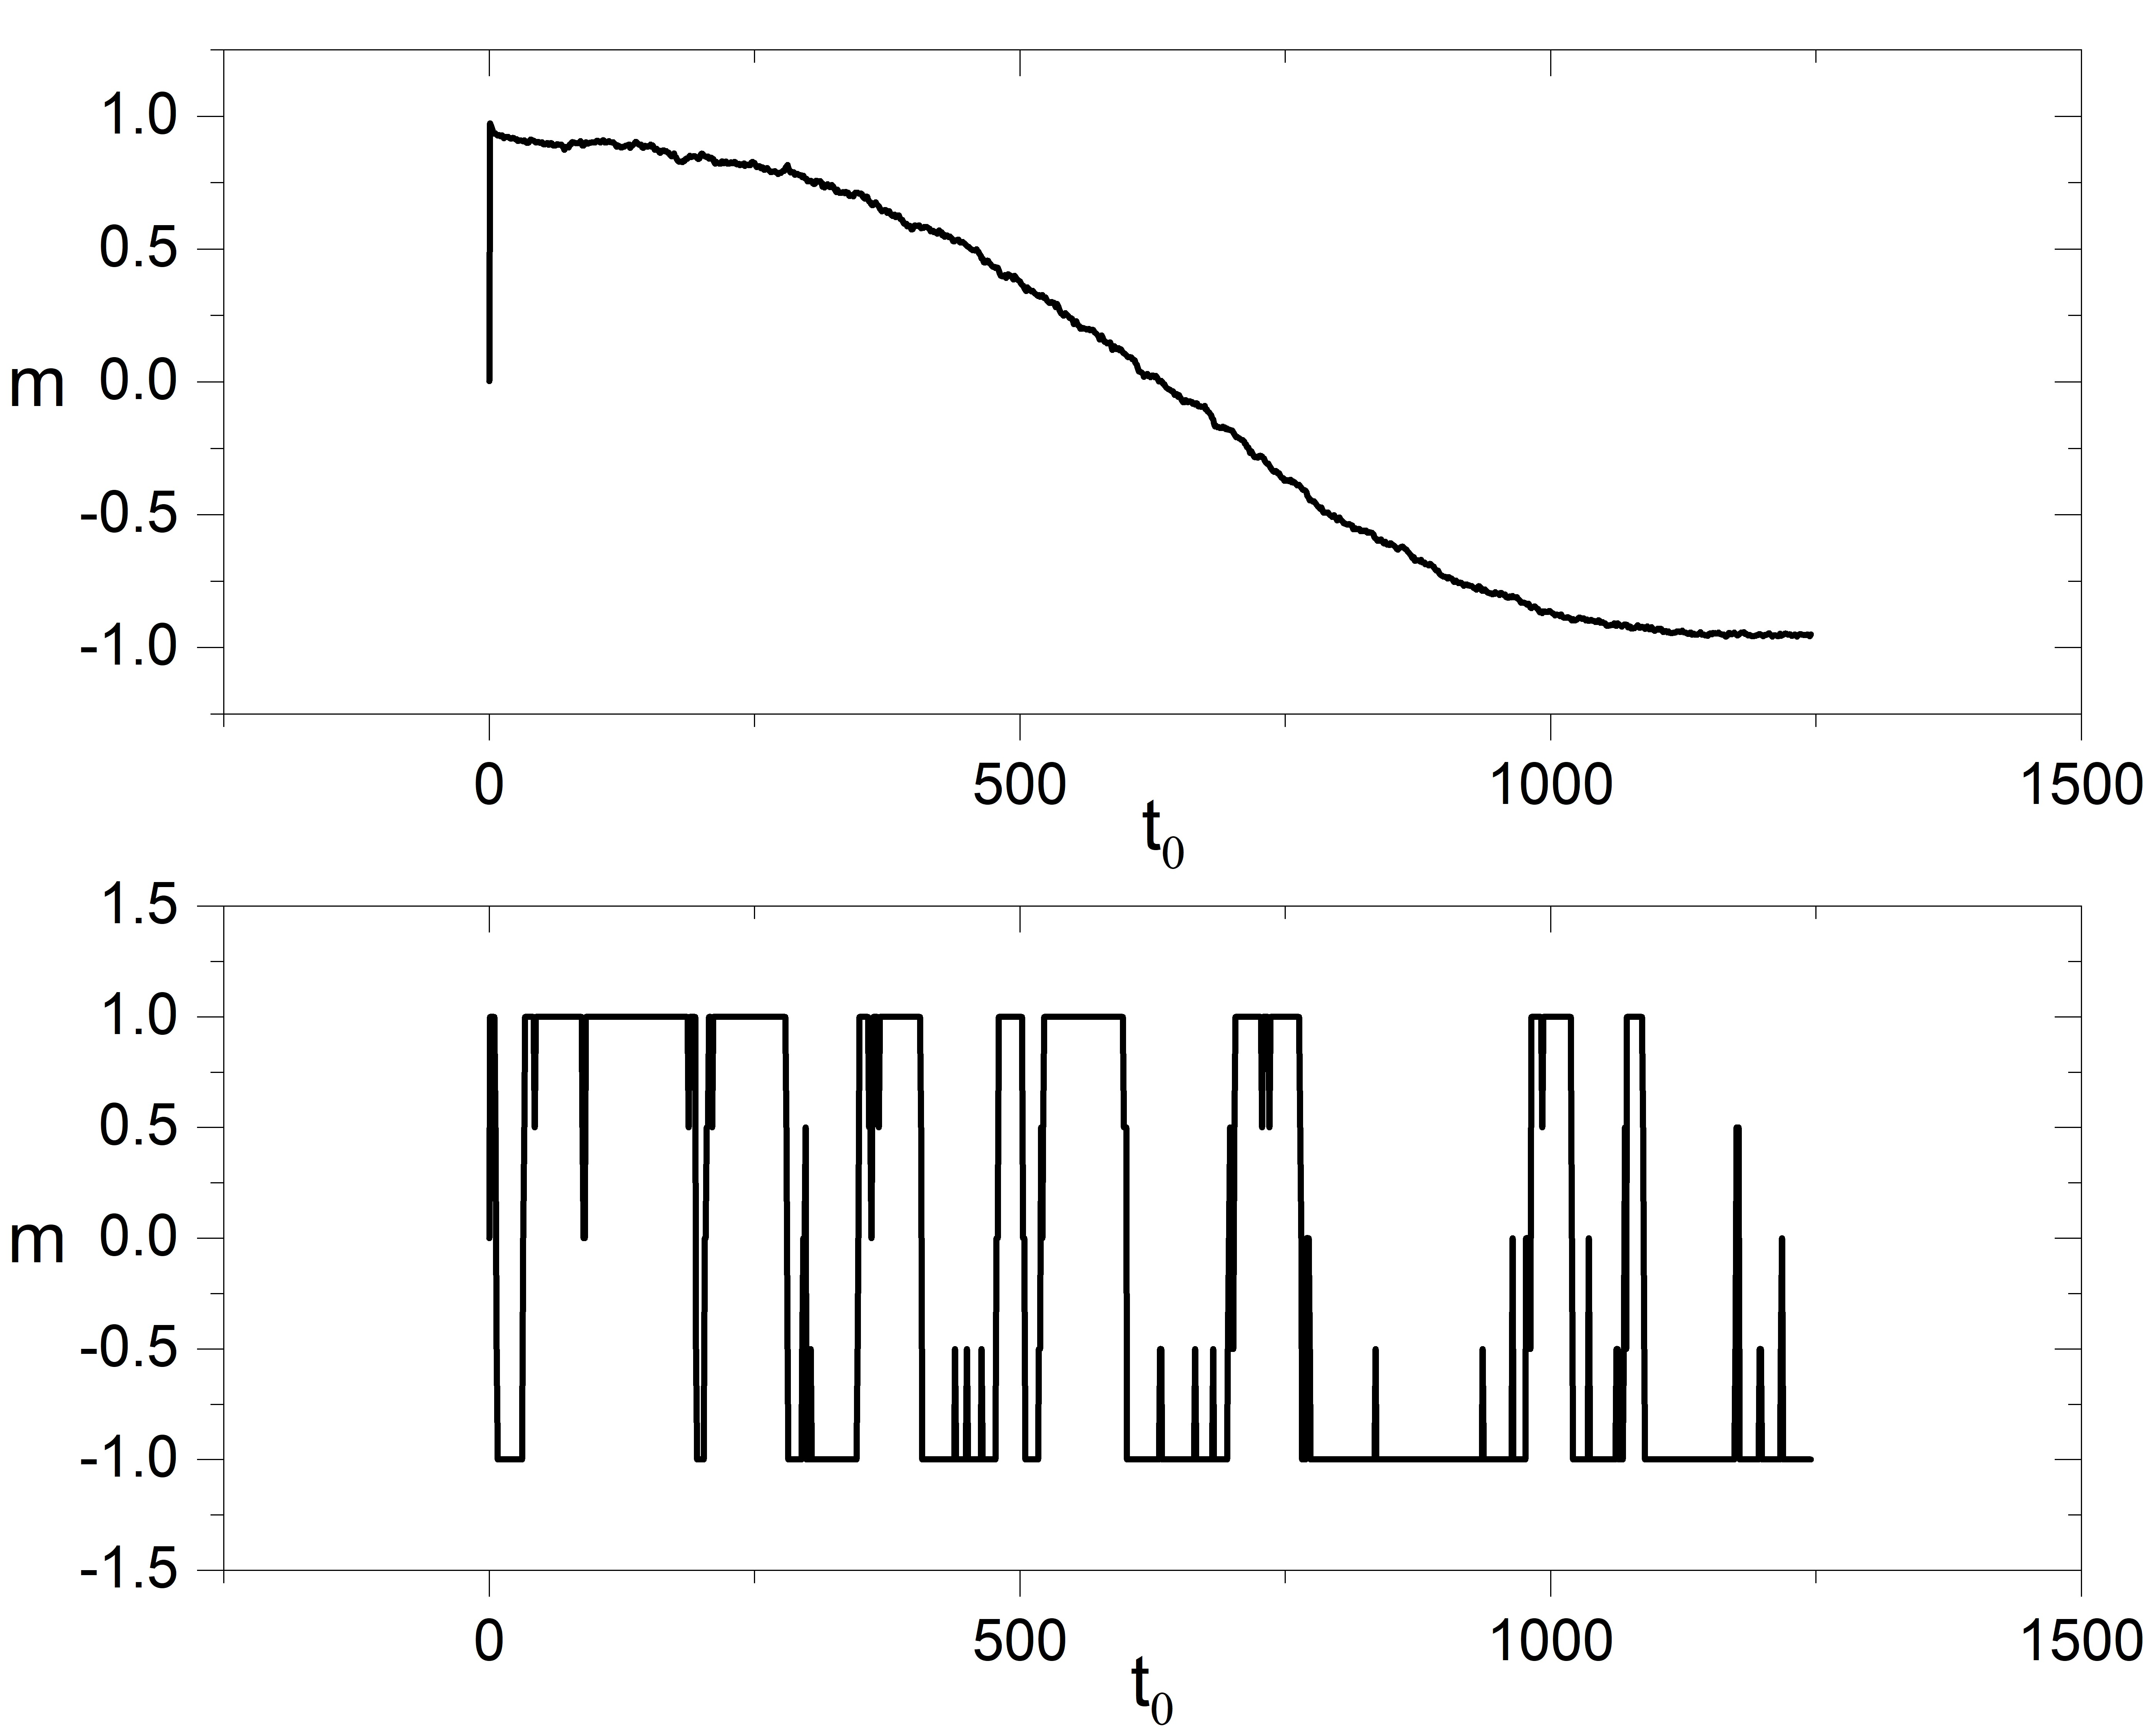
\includegraphics[width=\linewidth]{2x250x50mag.jpg}
\footnotesize
Figure 1. The magnetization m against time $t_{0}$, a characteristic time for the simulation, for a system size $N_{x}=N_{y}=100$ versus $N_{x}=N_{y}=2$ shown at the top and bottom respectively.
\end{Figure}
\normalsize
\newline
\newline
%-------------------------------------------------

The maximum system size allowed by the simulation, $N_{x} = N_{y} = 250$, is not used since it is observed that coalescence effects become more prominent at sizes $N > 100$ This is not taken into account in our model. The case where a single cluster of critical size forms before taking over the system is considered. In a coalescence regime demonstrated in Figure 2, two distinct gradients for a sufficiently large field is expected. This effect is not observed for $N_{x} = N_{y} = 100$ in our range of values. 
%-------------------------------------------------
% FIGURE 2
\newline
\newline
\begin{Figure}
\centering
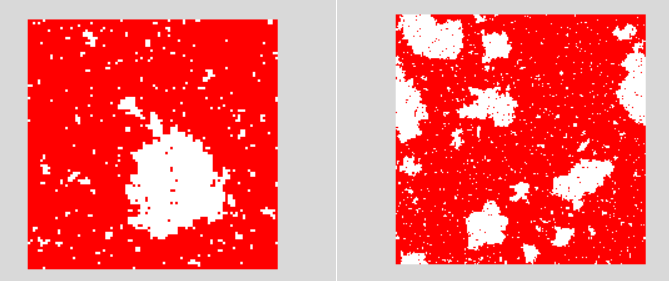
\includegraphics[width=\linewidth]{100vs200coalescence.png}
\footnotesize
Figure 2. Snapshots from the simulation at an initial external applied field of h= -0.1J for a system size $N_{x}=N_{y}=100$ shown on the left and $N_{x}=N_{y}=200$ shown on the right hand side, until nucleation or coalescence starts to occur respectively.
\end{Figure}
\normalsize
\newline
%-------------------------------------------------

A variation of preset 5 \cite{SSS} in the simulation is used to investigate the relationship between nucleation time $\tau_{crit}$ and the applied field h. The external field is varied from -0.12J to -0.30J in step-sizes of 0.01J. In the simulation, a value of 2J implies an external field strength $H = \frac{2J}{\mu}$ in units of Tesla, where $\mu$ represents the magnetic moments of the spins. The simulation uses units of time $t_{0}$ representing the characteristic time for relaxation of a spin to its own local field. As such it is difficult to compare this to more convenient units of time, i.e seconds [s]. We introduce a quantity $\epsilon$ which acts as a conversion factor between the units of time in the simulation and units of seconds [s] for nucleation time. Note this will not effect the relationship predicted by the theory. Let $\tau_{crit}=\epsilon\tau_{0}$ where $\tau_{0}$ is the nucleation time $\tau_{crit}$ in units of time [$t_{0}$] used by our simulation. Similarly introduce $h = \alpha h_{0}$ where $\alpha$ is a conversion factor and $h_{0}$ represents the applied external field in units of [J], the exchange constant between nearest neighbours. The new relationship can be written as
\begin{equation}\label{empirical log equation}
log(\tau_{0})=\frac{\gamma}{h_{0}}+ \delta
\end{equation}
where $\gamma$ and $\delta$ are constants of proportionality. This is verified by the results, as shown in Figures 3 and 4. A linear relationship is seen between the natural logarithm of the nucleation time $\tau_{0}$ and the applied external field $h_{0}$. The $y$ intercept given by the line of best fit is $3.00\pm0.04$ for the $100 \times 100$ system. Although the theory predicts a $y$ intercept of 0, a non-zero intercept is expected from the simulation due to the conversion for the units of time and inverse magnetic field. \newline

%-------------------------------------------------
% FIGURE 3
\newline
\begin{Figure}
\centering
\includegraphics[width=\linewidth]{100x100graph.jpg}
\footnotesize
Figure 3. The logarithmic relationship between the nucleation time $\tau_{0}$ and the inverse of the applied field $h_{0}$ for a system size of $N_{x} = N_{y} = 100$. The line of best fit has a gradient of $-0.40 \pm 0.01$. Some error bars are small and are hidden by the square tick marks. These errors can be seen more clearly in figure 5.
\end{Figure}
\normalsize
%-------------------------------------------------

Figure 4 shows the results for a system size of $N_{x}=N_{y}=50$. The simulation has been run with the same initial condition and range of values of the external applied field h used to plot Figure 3 to find the nucleation time $\tau_{0}$. Between the values of -8 and -7 of the inverse field $\frac{1}{h_{0}}$ there are 2 values which are significantly further away from the line of best fit than all the other data points. Directly comparing this to Figure 3 reveals that for a larger system size the data points are grouped closer around the line of best fit. 
%-------------------------------------------------
% FIGURE 4
\newline
\begin{Figure}
\centering
\includegraphics[width=\linewidth]{50x50raph.jpg}
\footnotesize
Figure 4. The logarithmic relationship between the nucleation time $\tau_{0}$ and the inverse of the applied field $h_{0}$ for a system size of $N_{x}=N_{y}=50$. The gradient of the line is $-0.40 \pm 0.02$.
\end{Figure}
\normalsize
\newline
\newline
%-------------------------------------------------

Figure 5 shows a plot of the error $\frac{\Delta x}{2}$ against the inverse applied field $\frac{1}{h_{0}}$. As some error bars are hidden by our tick markers, plotting the error directly for both systems at each value of $\frac{1}{h_{0}}$ gives a clearer distinction between the relative sizes of errors in our measurements for both systems. Overall the size of the error is reduced and our results are more consistent. The deviation from the mean is decreased with a larger system size. In this case it is $N_{x}=N_{y}=100$ versus $N_{x}=N_{y}=50$. For smaller values of $h_{0}$ the error for both systems is larger, but approaches 0 as the external applied field increases.
%-------------------------------------------------
% FIGURE 5
\newline
\newline
\begin{Figure}
\centering
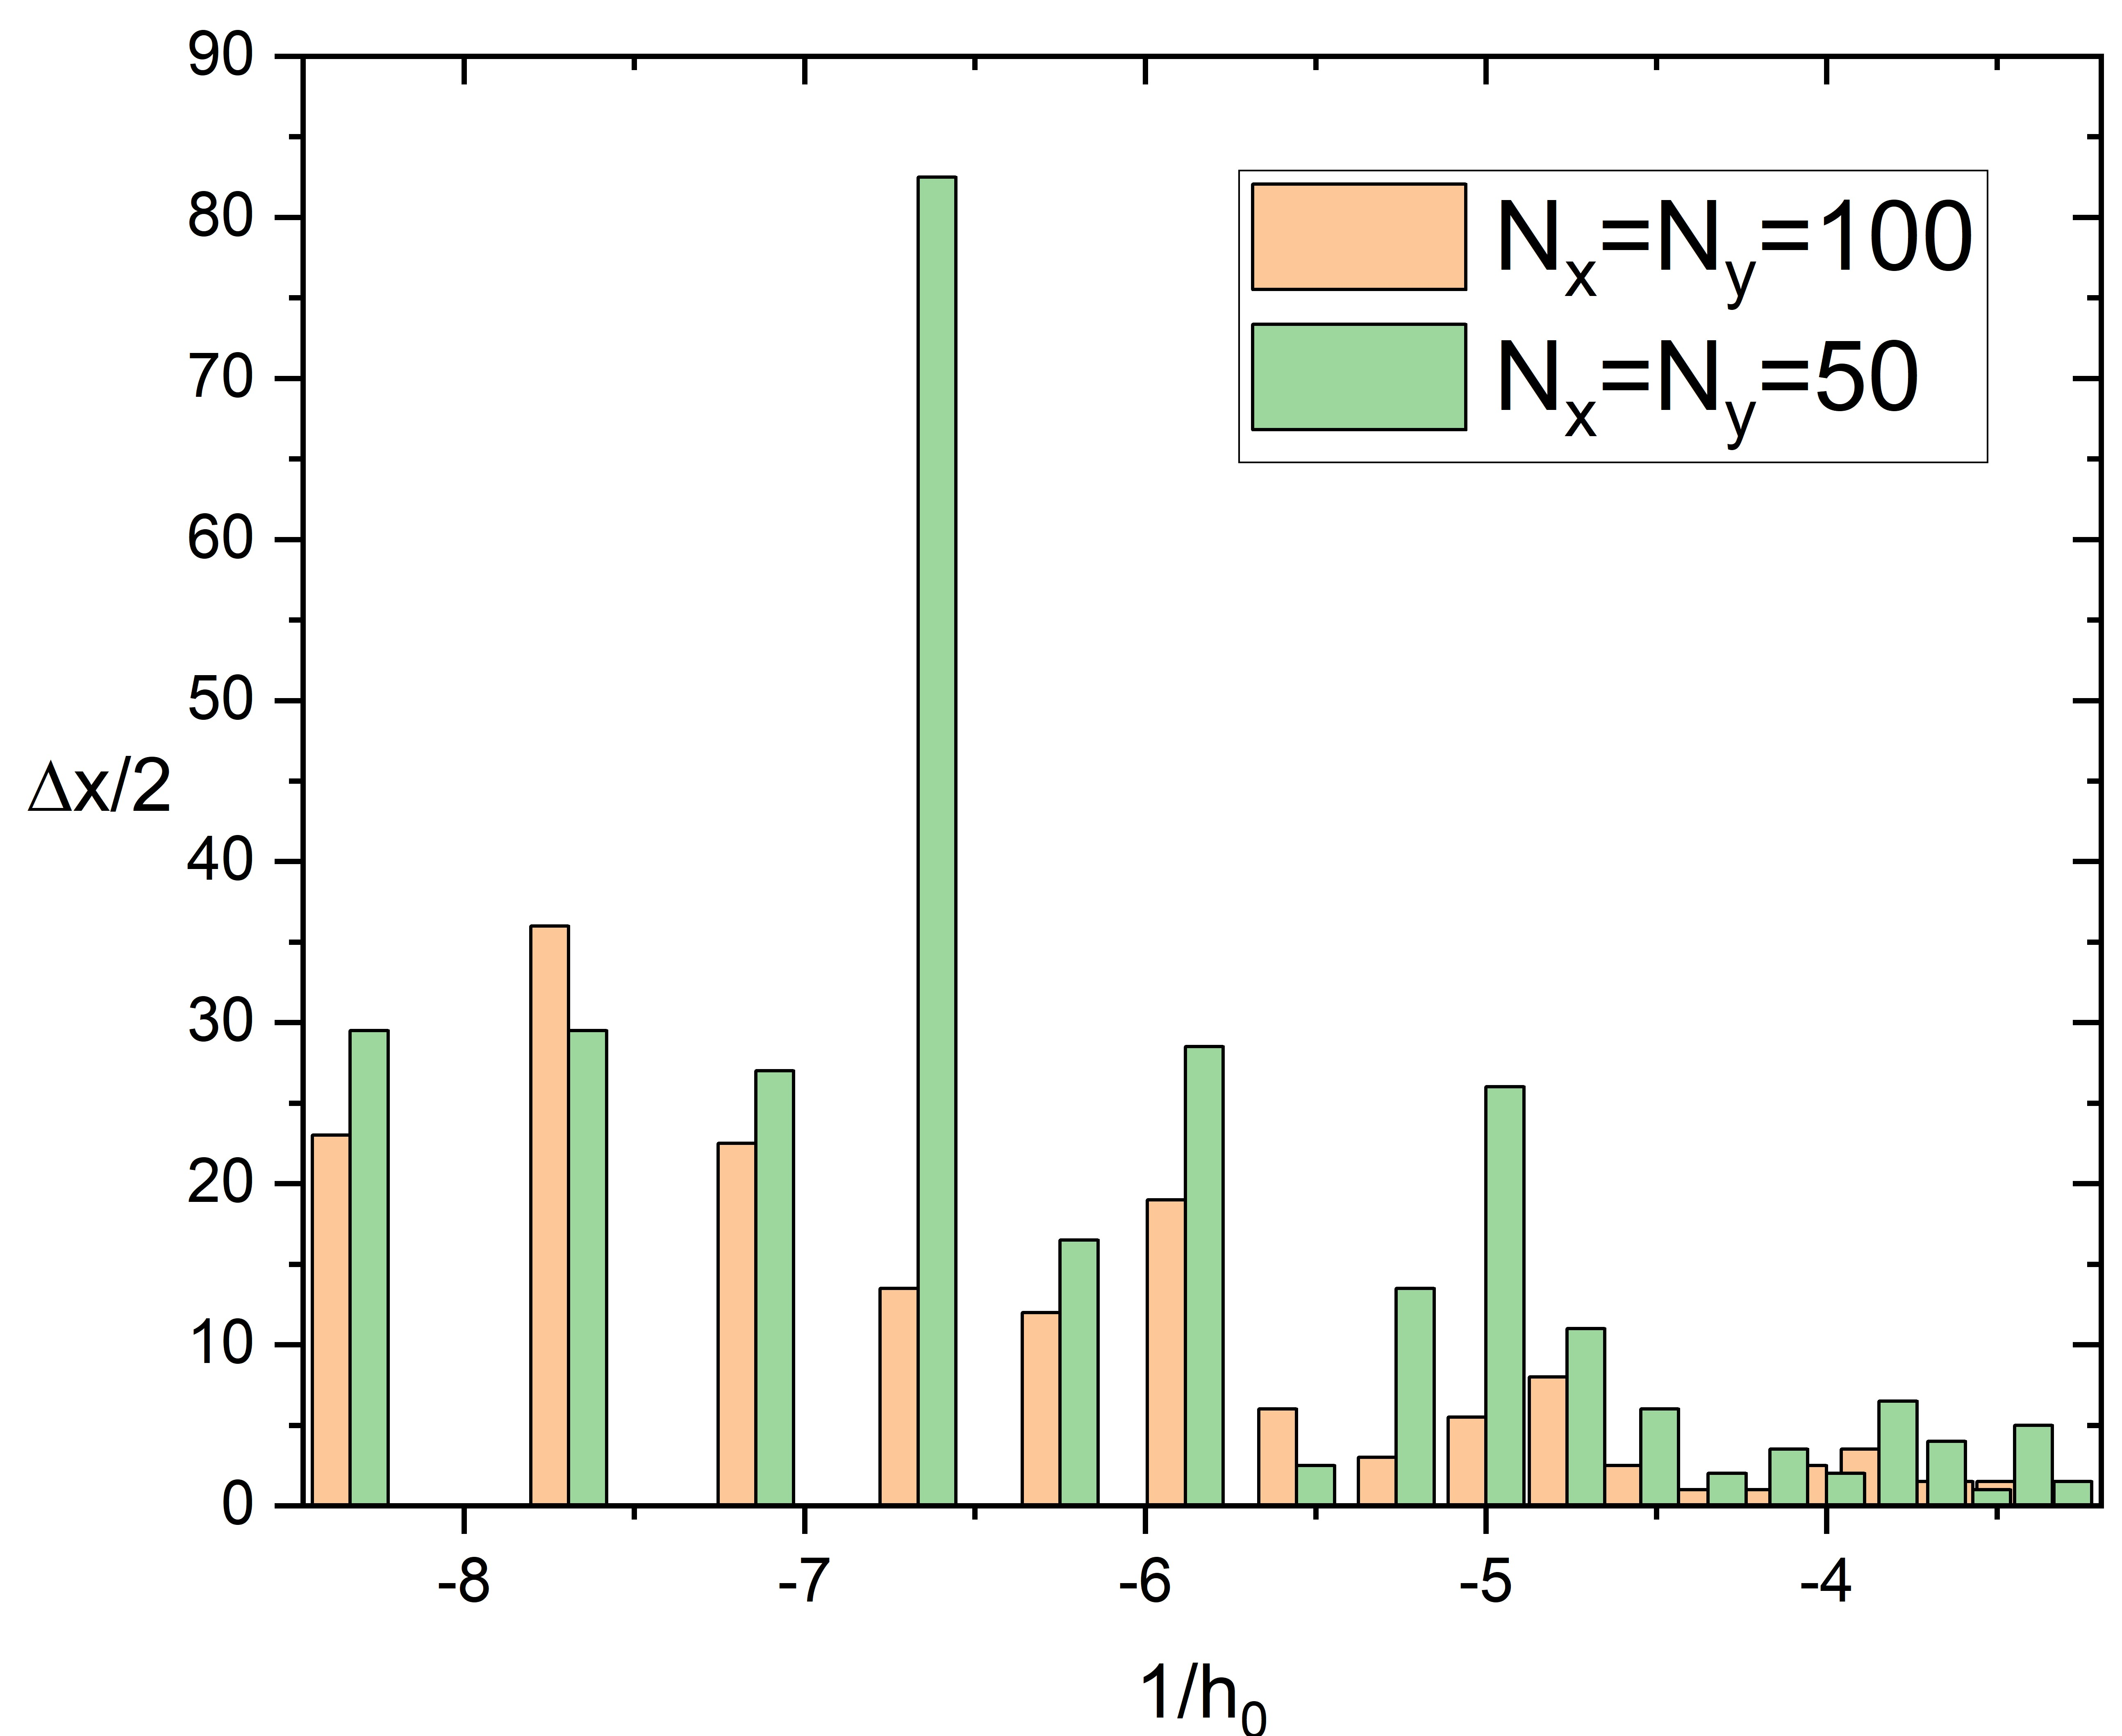
\includegraphics[width=\linewidth]{errorgraph.jpg}
\footnotesize
Figure 5. The error $\frac{\Delta x}{2}$ is plotted against the inverse applied field $\frac{1}{h_{0}}$ for a system size $N_{x}=N_{y}=100$ and $N_{x}=N_{y}=50$
\end{Figure}
\normalsize
%-------------------------------------------------
\maketitle
\section{Discussion}

By demonstrating the linear relationship between $log(\tau_{crit})$ and $\frac{1}{h}$, the Boltzmann distribution of nuclei size from CNT is recovered. However, there is still deviation from the straight line for large negative values of $\frac{1}{h}$ which must be accounted for. This may be a characteristic of the simulation, since at smaller fields it is harder for a nucleus of critical size to form, leading to greater variation. More measurements would need to be taken to see if these deviations would be reduced.

Our work has not taken coalescence into account, a more complicated regime dependent on the dimension of the system \cite{naskar_fields}. Further work is needed to investigate if we can still recover a Boltzmann distribution from Becker-Döring assumptions with stronger external fields.

In the context of epidemiology, we have drawn a parallel between the critical size for nucleation and the critical infection ratio for an epidemic outbreak, but our work does not explain whether a Boltzmann distribution for the critical infection ratio for an epidemic outbreak is realistic. Investigations into epidemiology sometimes make no mention of any underlying Boltzmann distribution in a population and instead implement a SIR model on a d-dimensional lattice, which still gives good agreement between the numerical and
the experimental epidemiological data \cite{liccardo}. Further studies are needed to see if the match between the Boltzmann distribution and reality is a coincidence or signifies something deeper.

During the onset of an epidemic, there are many factors to consider, including age group and household size \cite{liccardo}. CNT and the Ising model may be too simplistic. A step towards a more realistic model may be to include a dipolar interaction energy. For a 2D array with spins perpendicular to the plane, the dipolar magnetic field due to a spin-up state at one point is directed down at all other points in the lattice in order to favour the anti-parallel alignment of a pair of spins. Each spin interacts with all other spins in the lattice. Assuming a power law of $n = 3$, the Hamiltonian of the system would become
\begin{equation}\label{Hamiltonian_neel}
H = -J\sum_{<i,j>}S_{i}S_{j} - h\sum_{i}S_{i} + \frac{1}{2}\sum_{i,j}\frac{Da^{3}}{r_{ij}^{3}}S_{i}S_{j}
\end{equation}
where $D$ is the strength of the dipole-dipole interaction, $r_{ij}$ is the distance between lattice points $i$ and $j$, and $a$ is some lattice constant of the system \cite{SSS}. A parallel could be drawn between this extra term and the fact that people may travel within their communities, potentially infecting people further afield and not just their nearest neighbours, accounting for an extra factor. This would require a new simulation that incorporates this extra interaction between lattice points.




\printbibliography

\end{multicols*}
\end{document}
